\chapter{Ontwerpen}

\textit{In dit hoofdstuk zal er nagedacht worden over hoe de architectuur van her Proof of Concept er uit gaat zien. Alvorens dit opgesteld wordt dient er een methode gekozen te worden om het ontwerp mee te creëren. Na de totstandkoming van de keuze zullen de user-stories uitgewerkt worden. Deze user-stories zullen gebruikt worden voor de planning van de verschillende sprints tijdens de realisatie van het Proof of Concept.}

\section{Methode}

Het modelleren, implementeren en documenteren van een systeem vereist dat het systeem vanuit verschillende perspectieven wordt bekeken. Het is dan ook essentieel om een methode te selecteren die hiervan gebruik maakt. Er zullen twee methodes bekeken worden namelijk de methode van \cite{rozanski2012software}, waar ervaring mee opgedaan is tijdens de studie en de methode van \cite{kruchten19954+}, wat aangeraden is door mijn begeleider bij Quintor.

\subsection{\citeauthor{kruchten19954+}}

\begin{wrapfigure}{r}{0.6\textwidth}
    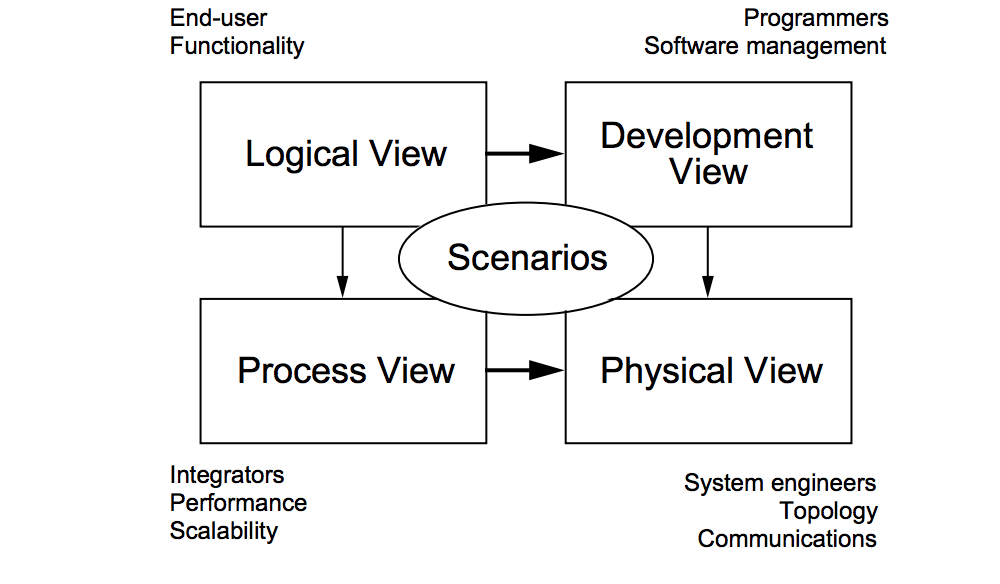
\includegraphics[width=0.6\textwidth, keepaspectratio]{figures/4+1}
    \caption[4+1 view-model]{Het 4+1 view-model volgens \cite{kruchten19954+}.}
    \label{architecture:kruchten}
\end{wrapfigure}  

Het 4+1 view-model organiseert een beschrijving van een software-architectuur met behulp van vijf views, die elk een specifieke reeks van problemen adresseren. Het is een lichter model als de methode van \cite{rozanski2012software} gezien het feit dat \cite{kruchten19954+} zich alleen richt op vier viewpoints. Dit is goed te zien in het overzicht van de methode in fig. \ref{architecture:kruchten}. Bij deze methode staan scenarios centraal en worden gebruikt tijdens het uitwerken van de vier viewpoints:

\paragraph{Development view} beschrijft het systeem uit het perspectief van een ontwikkelaar en beschrijft aspecten die te maken hebben met de software matige indeling.
\paragraph{Logical view} beschrijft hoe de eindgebruiker in staat zal zijn om de software te gebruiken. Hierbij worden vaak klassediagrammen en state diagrammen toegepast.
\paragraph{Process view} beschrijft de dynamische aspecten van het systeem op gebied van schaalbaarheid, integratie en performance.
\paragraph{Physical view} beschrijft hoe de softwarearchitectuur gaat werken op de benodigde hardware en focust zich met name op het gedistribueerde aspect ervan.

\subsection{\citeauthor{rozanski2012software}}

De methode van \cite{rozanski2012software} beschrijft de architectuur in zogenaamde viewpoints en perspectives. In deze viewpoints en perspectives zijn categorieën te vinden die elk verantwoordelijk zijn voor een aspect van de architectuur. Zo is er bijvoorbeeld het context-viewpoint waarin de relaties, dependencies en iteracties van het systeem met zijn omgeving wordt beschreven. De perspectives beschrijven de kwaliteitsattributen van een architectuur, waarbij het bijvoorbeeld gaat over accessibility of security.

\subsubsection{Keuze}

Door het aanraden van het 4+1 model door mijn begeleider en omdat het opstellen van de methode minder tijd zal kosten aangezien het minder omvang heeft als de methode van \cite{rozanski2012software}, is er besloten om gebruik te maken van het 4+1 model beschreven door \cite{kruchten19954+}.

\clearpage

\section{Opstellen scenarios}

Om een sprintplanning te maken is het benodigd om user-stories op te stellen voor het Proof of Concept. In de methode van \cite{kruchten19954+} wordt dit gedaan door het opstellen van use cases in het onderdeel scenario's, dat ook wel de use case view wordt genoemd. Voor het opstellen van de scenario's zal ik allereerst requirements opstellen, aangezien die benodigd zijn voor het uitwerken van de use cases. Omdat er geen stakeholder is die de rol van eindgebruiker invult, is het niet mogelijk om een interview af te nemen voor het elliciteren van de requirements. Om deze reden heb ik dan ook de requirements uit de informatie van het gedane onderzoek gehaald die de werking van de segmenten beschrijft.

Bij het opstellen van de requirements is er onderscheid gemaakt tussen non-functional en functional requirements. De non-functional requirements beschrijven de kwaliteitsattributen van het systeem, en de functional requirements beschrijft de werking van het systeem. Hieronder is een voorbeeld gegeven van een non-functional requirement die opgesteld is: \\

\begin{formal}
    ``Het systeem dient makkelijk uitgebreid te worden door de kerncompomenten modulair op te stellen.''
    \\ \textit{Non-functional requirement om de eis ``generiek'' te beschrijven, te vinden in het \nameref{appendix:architectuur}.}
\end{formal}

\begin{wrapfigure}{l}{0.6\textwidth}
    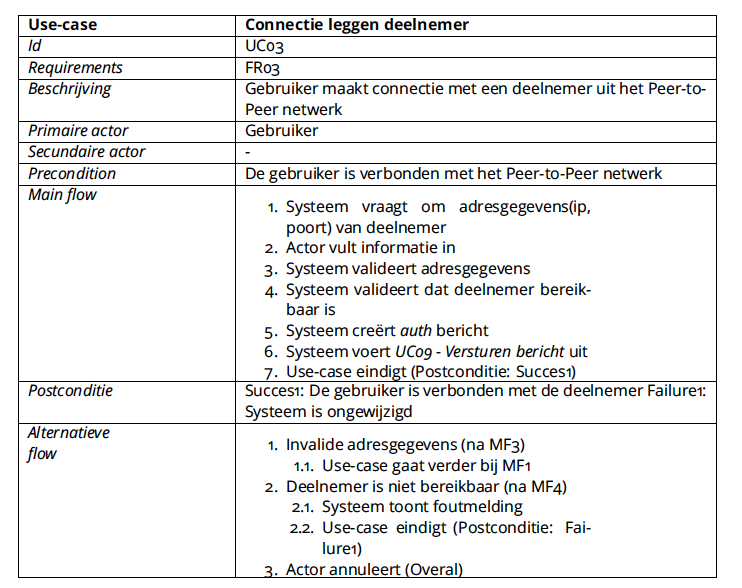
\includegraphics[width=0.6\textwidth, keepaspectratio]{figures/use-case}
    \caption[Voorbeeld use-case: Connectie leggen deelnemer]{Voorbeeld van een opgestelde use-case zoals te vinden in het \nameref{appendix:architectuur}.}
    \label{architecture:use-case}
\end{wrapfigure}  

Uiteindelijk heb ik de use cases opgesteld voor de functional requirements. Een voorbeeld hiervan is te zien in \ref{architecture:use-case}. De format die voor de use case beschrijving is gebruikt komt uit een school project waarin les gegeven is door dhr. John Smeets, een uitstekend docent op het gebied van UML. In \ref{architecture:use-case-diagram} is een overzicht te zien van alle gerealiseerde use cases en de relaties onderling. Zo wordt bijvoorbeeld de use case ``bericht versturen'' gebruikt in bijna elk andere use case omdat dit een van de kern functionaliteit is binnen het segment Distributed Network.

\clearpage

\begin{figure}
    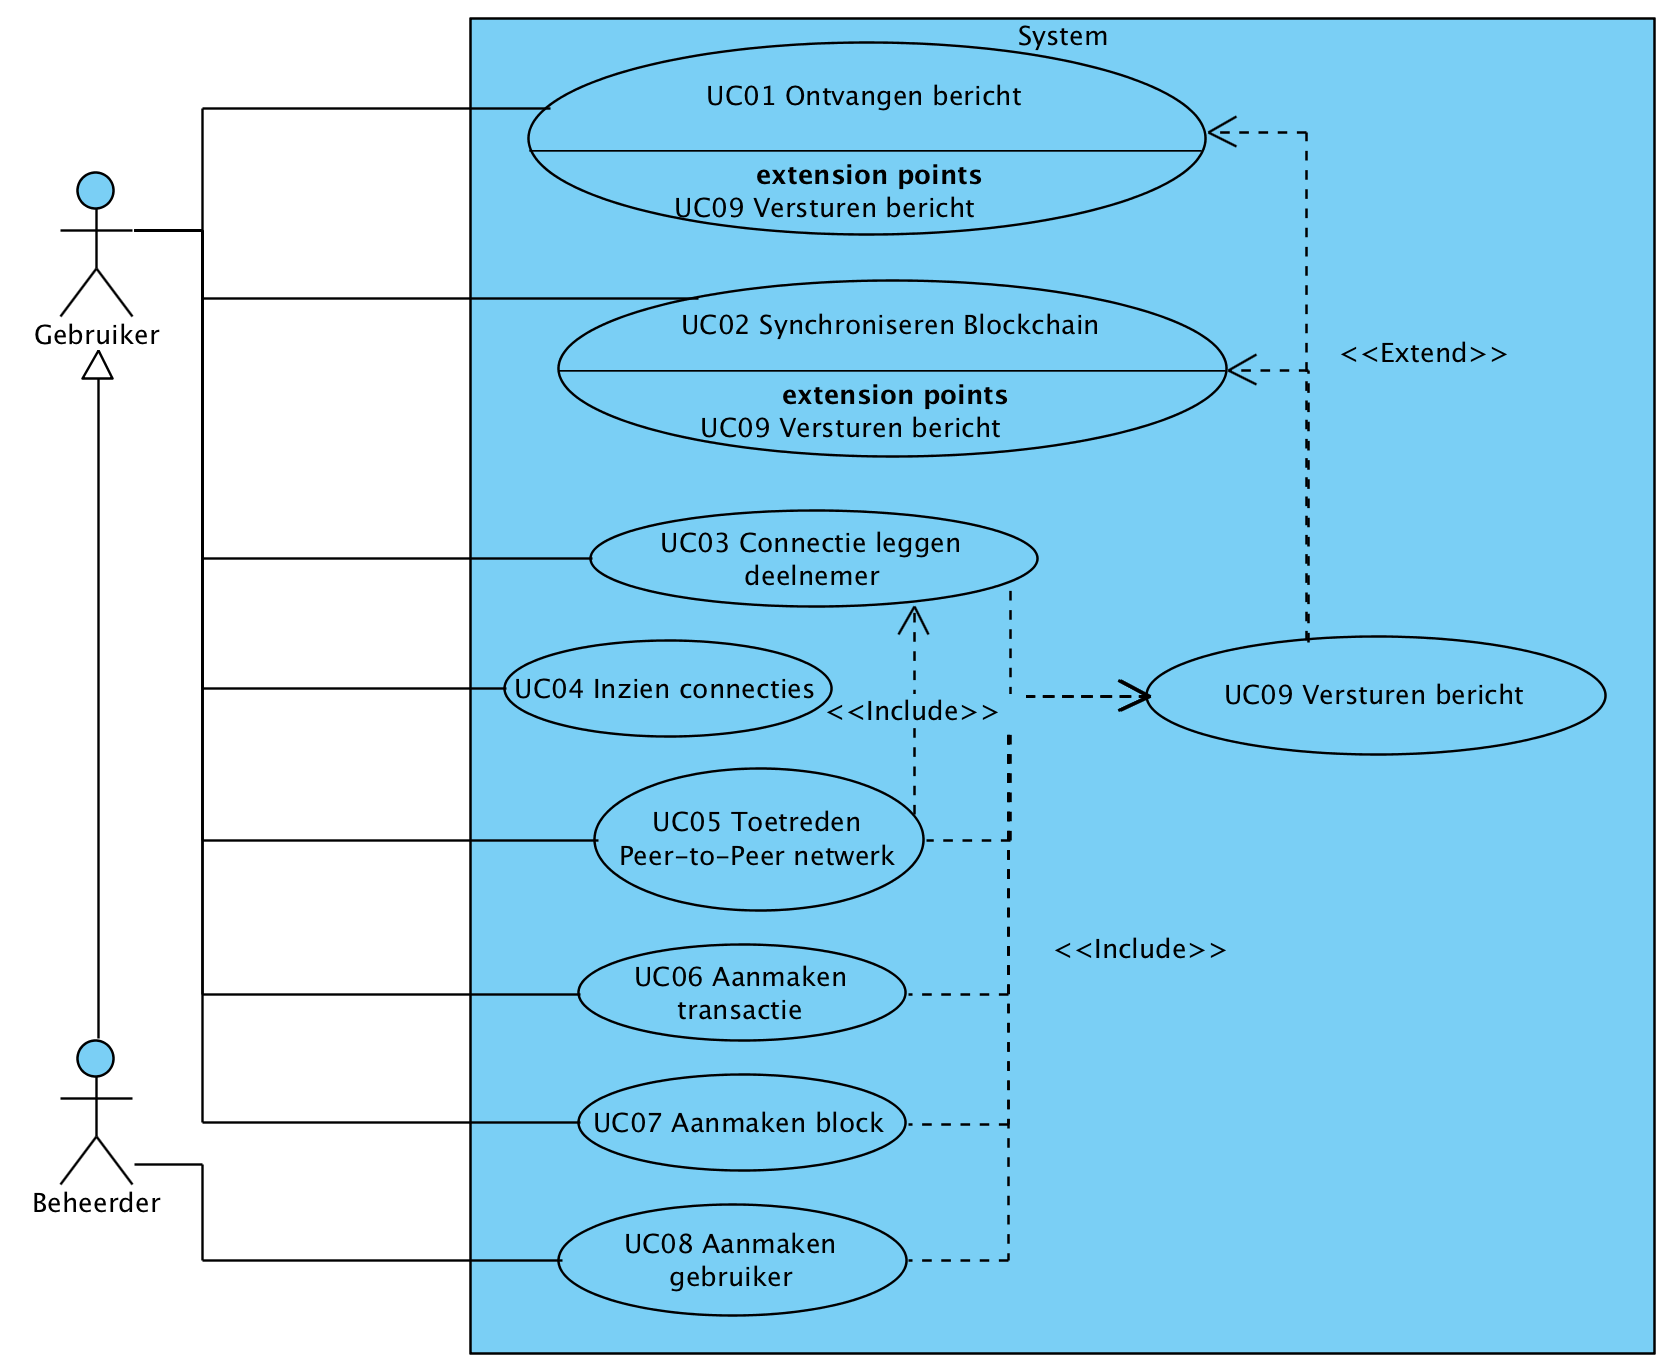
\includegraphics[width=\textwidth, keepaspectratio]{figures/use_case_diagram}
    \caption[Use-case diagram]{Totaalplaatje opgestelde use case diagrams}
    \label{architecture:use-case-diagram}
\end{figure}

\section{Development View}

Nu ik duidelijk weet welke functionaliteiten er in het systeem komen, kan ik beginnen aan de Development View. Hierin wordt het systeem beschreven in het perspectief van een ontwikkelaar waarin nagedacht wordt over de software matige indeling. Deze view zal ik als referentie gebruiken tijdens de realisatie van het Proof of Concept. Het uiteindelijke resultaat is te vinden in fig. \ref{architecture:component-diagram}. Elk component heeft een specifieke taak binnen de architectuur, waarbij voorbeeld het Discovery component verantwoordelijk is voor de Peer Discovery strategie die gebruikt zal worden. Een uitgebreide beschrijving van de componenten is te vinden in het \nameref{appendix:architectuur} document. 

\clearpage

\begin{figure}[h]
    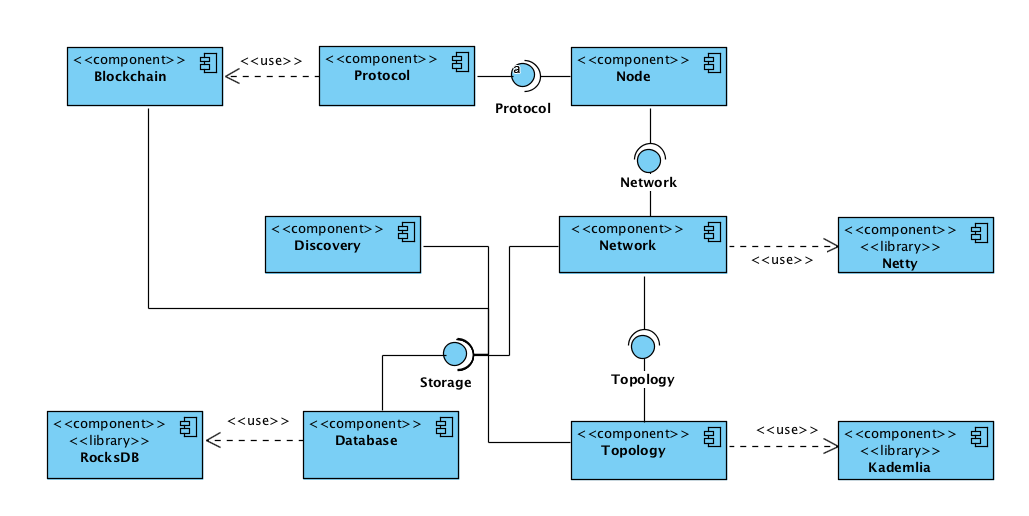
\includegraphics[width=\textwidth, keepaspectratio]{figures/component_diagram}
    \caption[Development View]{Development view van de te realiseren applicatie, waarin de interacties tussen de componenten in de vorm van interfaces weergegeven worden.}
    \label{architecture:component-diagram}
\end{figure}